\documentclass{article}
\usepackage{xeCJK}
\usepackage{amsmath}
\usepackage{listings}
\usepackage{xcolor}
\setlength{\parindent}{0pt}
\renewcommand{\baselinestretch}{1.0}
\usepackage[justification=centering]{caption}
\lstset{
	frame=tb, % draw a frame at the top and bottom of the code block
	showstringspaces=false, % don't mark spaces in strings
	numbers=left, % display line numbers on the left
	commentstyle=\color{green}, % comment color
	keywordstyle=\color{blue}, % keyword color
	stringstyle=\color{red} % string color
}
\usepackage[a4paper,left=20mm,right=20mm,top=15mm,bottom=15mm]{geometry}  

\title{Palindromic Tree}
\author{MengChunlei}

\begin{document}
\maketitle
\section{算法目标}
这个数据结构是用来辅助解决跟回文字符串相关的一些问题. 它的输入是一个字符串, 它的输出是一棵树. 树的具体定义如下面所描述.
\section{树的定义}
树包含很多节点.每个节点代表一个回文串.不同的节点代表的回文串是不同的. 节点上有两种边. 第一种称作$sonedge$(后面用实线表示), 它表示在当前字符串两边加上某个字符所对应的回文串的节点. 第二种称作$failedge$(后面用虚线表示), 它指向这个节点代表的回文串的最长的后缀回文串代表的节点.如下图所示: \par

\begin{figure}[h]
\centering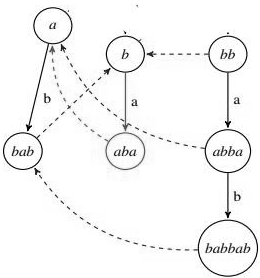
\includegraphics[scale=0.6]{pic1.png} \par
\end{figure}
另外, 节点$a$, $b$没有$failedge$. 为了完整性, 再增加一个虚拟节点, 表示长度为0的空串.  \par
\begin{figure}[h]
\centering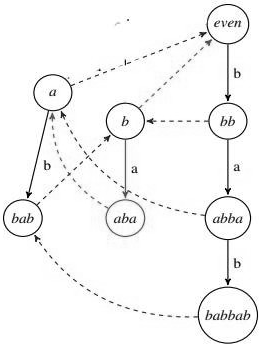
\includegraphics[scale=0.6]{pic2.png} \par
\end{figure}

这个长度为0的节点也叫做偶树根, 因为它所有的孩子节点所代表的回文串的长度都是偶数. 所以如果再有一个奇树根, 那么看起来很完美了. 这个奇树根的长度应该是-1, 因为它的孩子的长度应该比它大2. 加上奇树根后, 这个树如下所示:\par

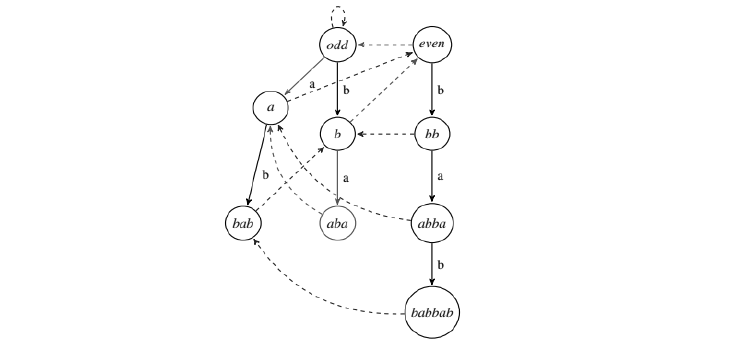
\includegraphics[scale=0.6]{pic3.png} \par

除了边以外, 每个节点会保存长度. 所以节点的定义如下所示:\par
\begin{lstlisting}[language=C++, caption={Node Definition}]
struct Node {
  std::array<Node*, N> sons;
  Node* fail;
  int len;
};
\end{lstlisting}
注意这里奇树根的长度为$-1$, 偶树根的长度为0. 偶树根的$failedge$指向奇树根(这个会利于后面的代码实现).奇树根的$failedge$指向它自己(这个没什么用).

\section{树的构造}
整个构造的过程是增量的.
初始化, 有两个节点, 即奇树根和偶树根. 同时保存$last$节点,它表示以插入的最后一个字符结尾的最长回文串的节点. 初始时$last=$偶树根, 表示初始时是一个空串. \par
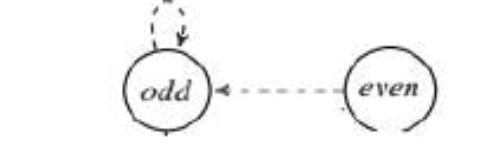
\includegraphics[scale=0.4]{pic4.png} \par

假设已经构造了一个串的前$p-1$个字符的树.且以$s[p-1]$结尾的最长回文串的节点为$last$. 现在考虑第$p$个字符,$s[p]$ .目的是创建(或找到)以$s[p]$结尾的最长回文串的节点. 首先, 如果$last$满足$s[p-last.len-1]=s[p]$, 那么说明$s[p-last.len-1]\rightarrow  s[p]$是回文的(如下图所示的红色方框) \par
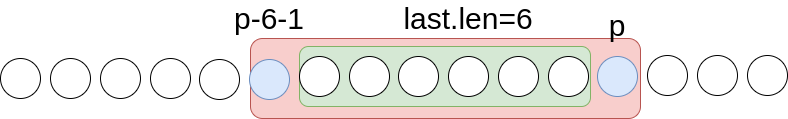
\includegraphics[scale=0.6]{pic5.png} \par
如果$s[p-last.len-1]\neq s[p]$, 那么需要找到$last$代表的回文串的最长后缀的回文串节点$target$, 并且满足$s[p-target.len-1]=s[p]$. 这正是$failedge$的定义. 所以寻找$target$的方法如下:
\begin{lstlisting}[language=C++, caption={FindTarget}]
Node* FindTarget(Node* last, const std::string &s, size_t p) {
  Node* target = last;
  while (s[n - target->len - 1] != s[p]) {
    target = target->fail;
  }
  return target;
}
\end{lstlisting}
这里可以看到, 如果一直沿着$faledge$向上找, 那么最终会到达奇树根, 而它的长度为$-1$,这时候一定满足$s[p-(-1)-1]=s[p]$.这也是奇树根长度为$-1$的好处.
找到了$target$之后, 有两种情况: \par
第一种情况, $target$已经有一个为$s[p]$的孩子, 即$target.sons[s[p]]\neq nullptr$, 这说明之前已经出现过同样的回文串. \par
~\\
第二种情况, $target.sons[s[p]]= nullptr$, 这时候需要新建一个节点来表示回文串$s[p-target.len-1]\rightarrow  s[p]$, 令这个节点为$curr$, 那么有$target.sons[s[p]]=curr, curr.len=target.len + 2$. 现在考虑$curr.fail$是什么.跟上面同样的道理, $curr.fail$所代表的回文串如果去掉两边的两个字符, 那么剩下的回文串一定是$target.fail$或者$target.fail.fail$或者$target.fail.fail.fail$等等.所以还是可以调用$FindTarget$去找到一个满足条件的节点. \par
~\\
所以新插入字符的实现如下:
\begin{lstlisting}[language=C++, caption={Append}]
Node* Append(cnost std::string &s, size_t p, Node* last) {
  Node* target = GetTarget(last, s, p);
  int index = s[p] - 'a'; 
  if (target->sons[index] == nullptr) {
    Node* curr = new Node();
    target->sons[index] = curr;
    curr->len = target->len + 2;
    curr->fail = GetTarget(target->fail, s, p)->sons[index];
  }
  return target->sons[index];
}
\end{lstlisting}
函数最后返回了以新插入的字符结尾的最长回文串对应的节点, 它应该作为新的$last$, 以便插入$s[p+1]$.

\section{复杂度}
可以证明, 对于一个长度为$n$的串$s$, 树的节点的个数最多为$n+2$. 插入$n$个字符的时间复杂度也是$O(n)$的.

\section{参考}
https://oi-wiki.org/string/pam/ \par
https://www.cnblogs.com/lhm-/p/13293090.html \par
https://blog.csdn.net/u013368721/article/details/42100363 \par

\end{document}
